\documentclass[a4paper]{article}
\usepackage{pgf,tikz,pgfplots}
\usetikzlibrary{arrows,decorations.markings}
\pgfplotsset{compat=1.15}
\usepackage{mathrsfs}
\usetikzlibrary{arrows}
%% Language and font encodings
\usepackage[english]{babel}
\usepackage[utf8x]{inputenc}
\usepackage[T1]{fontenc}
\usepackage{float}
%% Sets page size and margins
\usepackage[a4paper,top=3cm,bottom=2cm,left=3cm,right=3cm,marginparwidth=1.75cm]{geometry}
\usepackage{fancyhdr}
\pagestyle{fancy}
%% Useful packages

\usepackage{amsmath}
\usepackage{amsthm}
\usepackage{enumitem}
\usepackage{eqnarray}
\usepackage{float}
\usepackage{esint}
\usepackage{wrapfig}
\usepackage{gensymb}
\usepackage{lipsum}
\usepackage{amssymb}
\usepackage{array}
\usepackage{tikz}
\usepackage[colorlinks=true, allcolors=blue]{hyperref}
\usepackage{graphicx}
\usepackage{amsmath}
\usepackage{amssymb}
\usepackage{graphicx}
\usepackage[colorlinks=true, allcolors=blue]{hyperref}
\usepackage{mathtools}
\DeclareMathOperator{\Proj}{Proj}
\DeclareMathOperator{\lcm}{lcm}
\DeclareMathOperator{\cosec}{cosec}
\DeclareMathOperator{\sgn}{sgn}
\DeclareMathOperator{\Span}{span}
\DeclareMathOperator{\nullity}{nullity}
\DeclarePairedDelimiter\floor{\lfloor}{\rfloor}
\DeclareMathOperator{\Res}{Res}
\DeclareMathOperator{\rank}{rank}
\DeclareMathOperator{\Ker}{Ker}
\DeclareMathOperator{\R}{R}
\DeclareMathOperator{\Tr}{Tr}
\DeclareMathOperator{\diag}{diag}
\DeclareMathOperator{\Log}{Log}
\DeclareMathOperator{\sech}{sech}
\DeclareMathOperator{\Var}{Var}
\newtheorem{ans}{Answer}[section]

\definecolor{darkblue}{RGB}{	0, 0, 139}
\newtheoremstyle{new}% <name>
{2pt}% <Space above>
{2pt}% <Space below>
{\color{darkblue}}% Body font
{}% <Indent amount>
{\bfseries\color{black}}% Theorem head font
{:}% <Punctuation after theorem head>
{.5em}% <Space after theorem headi>
{}% <Theorem head spec (can be left empty, meaning `normal')>
\theoremstyle{new}
\newtheorem{qns}{Problem}[section]
\setlength{\parindent}{0cm}
\title{\textbf{Part II TSP Problem Sheet Solutions}}
\author{Tai Yingzhe, Tommy (ytt26)}
\date{}
\setlength{\parindent}{0cm}
\begin{document}
\maketitle
\tableofcontents
\newpage
\section{Problem Sheet 1}
\subsection*{Thermodynamics}
\begin{qns}[Van der Waals gas]
Show that, for a van der Waals gas, the specific heat at constant volume, $C_V$ , obeys 
$$\bigg(\frac{\partial C_V}{\partial V}\bigg)_T=0$$
\end{qns}
\begin{ans}
The heat capacity at constant volume is defined to be
$$C_V=\bigg(\frac{\partial U}{\partial T}\bigg)_V=T\bigg(\frac{\partial S}{\partial T}\bigg)_V$$
Take the partial derivative
$$\bigg(\frac{\partial C_V}{\partial V}\bigg)_T=T\bigg(\frac{\partial}{\partial T}\bigg)_V\bigg(\frac{\partial S}{\partial V}\bigg)_T=T\bigg(\frac{\partial^2p}{\partial T^2}\bigg)_V$$
where we used the Maxwell relation $(\frac{\partial S}{\partial V})_T=(\frac{\partial p}{\partial T})_V$. But the van der Waals equation of state is
$$p=\frac{Nk_BT}{V-Nb}-\frac{N^2a}{V^2}\implies\bigg(\frac{\partial p}{\partial T}\bigg)_V=\frac{Nk_B}{V-Nb}\implies\bigg(\frac{\partial C_V}{\partial V}\bigg)_T=T\bigg(\frac{\partial^2p}{\partial T^2}\bigg)_V=0$$
\end{ans}
\begin{qns}[Potentials and thermodynamic variables]
The Gibbs free energy of an imperfect gas containing $N$ molecules is given, in terms of its natural variables $T$, $p$ and $N$, by
$$G=Nk_BT\ln\frac{p}{p_0}-NA(T)p$$
where $p_0$ is a constant and $A$ is a function of $T$ only. Derive expressions in terms of $T$, $p$, $V$, and $N$ for:
\begin{enumerate}[label=(\alph*)]
\item the equation of state of the gas;
\item the entropy, $S$;
\item the enthalpy, $H$;
\item the internal energy, $U$;
\item the Helmholtz free energy, $F$.
\end{enumerate}
Can all equilibrium thermodynamic information about the gas be obtained from a knowledge of: (i) $F(T, V, N)$; (ii) the equation of state and $U(T, p, N)$?
\end{qns}
\begin{ans}
Note that $dG=-SdT+Vdp$. $G$ is thus given in terms of its natural variables so it is possible to deduce all thermodynamic properties.
\begin{enumerate}[label=(\alph*)]
\item To find the equation of state (function of $p$, $T$ and $V$), we have
$$V=\bigg(\frac{\partial G}{\partial p}\bigg)_{T,N}=\frac{Nk_BT}{p}-NA$$
\item The entropy is a conjugate variable with temperature
$$S=-\bigg(\frac{\partial G}{\partial T}\bigg)_{p,N}=-Nk_B\ln\frac{p}{p_0}+Np\bigg(\frac{\partial A}{\partial T}\bigg)_{p,N}$$
\item By definition, the enthalpy is
$$H=G+TS=Nk_BT\ln\frac{p}{p_0}-NA(T)p+T\bigg\{-Nk_B\ln\frac{p}{p_0}+Np\bigg(\frac{\partial A}{\partial T}\bigg)_{p,N}\bigg\}=Np\bigg(\bigg(\frac{\partial A}{\partial T}\bigg)_{p,N}T-A\bigg)$$
\item By definition, the internal energy is
$$U=H-pV=Np\bigg(\bigg(\frac{\partial A}{\partial T}\bigg)_{p,N}T-A\bigg)-(Nk_BT-NpA)=TN\bigg[p\bigg(\frac{\partial A}{\partial T}\bigg)_{p,N}-k_B\bigg]$$
\item By definition, the Helmholtz free energy is
$$F=U-TS=TN\bigg[p\bigg(\frac{\partial A}{\partial T}\bigg)_{p,N}-k_B\bigg]+TNk_B\ln\frac{p}{p_0}-NpT\bigg(\frac{\partial A}{\partial T}\bigg)_{p,N}=Nk_BT\bigg(\ln\frac{p}{p_0}-1\bigg)$$
\end{enumerate}
\begin{enumerate}[label=\roman*]
\item We have the free energy to be
$$dF=dU-d(TS)=-SdT-pdV+\mu dN$$
So, $T$, $V$ and $N$ are natural variables of $F$. Hence, all equilibrium thermodynamic information can be obtained.
\item Internal energy is however, $dU=TdS-pdV+\mu dN$ and so the natural variables of $U$ are $S$, $V$ and $N$. We need to change $T\rightarrow S$ and $p\rightarrow V$. But, the equation of state only allow one such change.
\end{enumerate}
\end{ans}
\begin{qns}[Entropy of the monatomic gas]
The entropy of a monatomic ideal gas is given by the Sackur-Tetrode equation which can be written in the form:
$$S(U,V,N)=Nk_B\ln\bigg\{\alpha\frac{V}{N}\bigg(\frac{U}{N}\bigg)^{3/2}\bigg\}$$
where $\alpha$ is a constant to be derived later in the course. Invert this expression to get $U(S, V, N)$. From this, obtain the equation of state expressing $p$ as a function of $V$, $N$ and $T$.
\end{qns}
\begin{ans}
Invert the expression:
$$S(U,V,N)=\frac{3}{2}Nk_B\ln\bigg\{\bigg(\alpha\frac{V}{N}\bigg)^{2/3}\frac{U}{N}\bigg\}\implies U(S,V,N)=e^{2S/3Nk_B}\bigg(\frac{N}{\alpha V}\bigg)^{2/3}N$$
But we have $dU=TdS-pdV+\mu dN$ and so
$$p=-\bigg(\frac{\partial U}{\partial V}\bigg)_{S,N}=\frac{2U}{3V},\quad T=\bigg(\frac{\partial U}{\partial S}\bigg)_{V,N}=\frac{2}{3Nk_B}U$$
which separately gives 
$$p=\frac{2}{3}U/V,\quad U=\frac{3}{2}Nk_BT$$
The latter is consistent with the equipartition of energy while the former
$$p=\frac{2}{3}\frac{3}{2}\frac{N}{V}k_BT\implies Nk_BT=pV$$
is consistent with the ideal gas law. $U$ is given in terms of its natural variables, so all thermodynamic properties can be deduced.
\end{ans}
\newpage
\begin{qns}[Analytic thermodynamics]
Use a Maxwell relation and the chain rule to show that for any substance the rate of change of $T$ with $p$ in a reversible adiabatic compression is given by
$$\bigg(\frac{\partial T}{\partial p}\bigg)_S=\frac{T}{C_p}\bigg(\frac{\partial V}{\partial T}\bigg)_p$$
Find an equivalent expression for the adiabatic rate of change of $T$ with $V$ , and check that both results are valid for an ideal monatomic gas.
\end{qns}
\begin{ans}
We have $dH=TdS+Vdp$, which gives the Maxwell relation
$$\bigg(\frac{\partial T}{\partial p}\bigg)_S=\bigg(\frac{\partial V}{\partial S}\bigg)_p=\bigg(\frac{\partial V}{\partial T}\bigg)_p\bigg(\frac{\partial T}{\partial S}\bigg)_p$$
But, $C_p=(\frac{\partial U}{\partial T})_p=T(\frac{\partial S}{\partial T})_p$, which gives our relation. Next, we want to find $(\frac{\partial T}{\partial V})_S$. We have $dU=TdS-pdV$, which gives the Maxwell relation
$$\bigg(\frac{\partial T}{\partial V}\bigg)_S=-\bigg(\frac{\partial p}{\partial S}\bigg)_V=-\bigg(\frac{\partial p}{\partial T}\bigg)_V\bigg(\frac{\partial T}{\partial S}\bigg)_V=-\frac{T}{C_V}\bigg(\frac{\partial p}{\partial T}\bigg)_V$$
where $C_V=(\frac{\partial U}{\partial T})_V=T(\frac{\partial S}{\partial T})_V$. For ideal gas, the equation of state is $pV=Nk_BT$. For an adiabatic process, $pV^\gamma=\text{const.}$ we have
$$0=d(pV^\gamma)=d[(Nk_BT)^\gamma p^{1-\gamma}]=\gamma T^{\gamma-1}p^{1-\gamma}dT+(1-\gamma)T^\gamma p^{-\gamma}dp$$
For monatomic gas, we have $\gamma=5/3$. We show:
$$\bigg(\frac{\partial T}{\partial p}\bigg)_S=-\frac{1-\gamma}{\gamma}\frac{T}{p}=\frac{2T}{5p},\quad \frac{T}{C_p}\bigg(\frac{\partial V}{\partial T}\bigg)_p=\frac{T}{2.5Nk_B}\frac{Nk_B}{p}=\frac{2T}{5p}$$
We can also write the adiabatic process as
$$0=d(pV^\gamma)=V^{\gamma-1}dT+TV^{\gamma-2}(\gamma-1)dV$$
which gives
$$\bigg(\frac{\partial T}{\partial V}\bigg)_S=-(\gamma-1)\frac{T}{V}=-\frac{2T}{3V},\quad -\frac{T}{C_p}\bigg(\frac{\partial p}{\partial T}\bigg)_V=-\frac{T}{1.5Nk_B}\frac{Nk_B}{V}=-\frac{2T}{3V}$$
\end{ans}
\begin{qns}[Brief Notes]
Write brief notes on thermodynamic equilibrium in closed and open systems.
\end{qns}
\begin{ans}
The thermodynamic equilibrium state is defined as the one macroscopic state of a system which is automatically attained after a sufficiently long period of time such that the macroscopic properties of the system no longer change with time. The governing principle of thermodynamic equilibrium is that the entropy of the Universe tends to a maximum.\\[5pt]
Closed systems does not exchange energy or particles with the environment. The entropy is maximized with respect to the internal constraints of the system. Consider a system of total energy $U$, total volume $V$ and total particle number $N$ with an imaginary wall that partitions the system into two regions of volumes $V_1$, $V_2$, energies $U_1$, $U_2$ and particle numbers $N_1$, $N_2$. Since the system is closed, we have
$$V_1+V_2=V,\quad U_1+U_2=U,\quad N_1+N_2=N$$
Maximize the total entropy $S=S_1+S_2$:
\begin{align}
    0&=dS_1+dS_2\nonumber\\&=\bigg(\frac{\partial S_1}{\partial U_1}\bigg)_{V_1,N_1}dU_1+\bigg(\frac{\partial S_2}{\partial U_2}\bigg)_{V_2,N_2}dU_2+\bigg(\frac{\partial S_1}{\partial V_1}\bigg)_{U_1,N_1}dV_1\nonumber\\&+\bigg(\frac{\partial S_2}{\partial V_2}\bigg)_{U_2,N_2}dV_2+\bigg(\frac{\partial S_1}{\partial N_1}\bigg)_{V_1,U_1}dN_1+\bigg(\frac{\partial S_2}{\partial N_2}\bigg)_{V_2,U_2}dN_1\nonumber\\&=\bigg(\frac{1}{T_1}-\frac{1}{T_2}\bigg)dU+\bigg(\frac{P_1}{T_1}-\frac{P_2}{T_2}\bigg)dV_1-\bigg(\frac{\mu_1}{T_1}-\frac{\mu_2}{T_2}\bigg)dN_1\nonumber
\end{align}
There are thus three types of equilibrium for a closed system:
\begin{itemize}
    \item thermal equilibrium: the temperatures of the two regions are the same. For constant volume and particle numbers, the system will evolve to this state by letting heat flow from the hotter region to the colder region.
    \item mechanical equilibrium: the pressures of the two regions are the same. For same temperature and particle numbers, the system will evolve to this state by moving the partition such that the higher pressure region expands into the other.
    \item chemical equilibrium: the chemical potential of the two regions are the same. For same temperature and volumes, the system will evolve to this state by allowing particles to flow down the chemical potential gradient.
\end{itemize}
We extend our arguments to an open system. Open systems allow heat and particle number exchange with the system and reservoir. The previous discussion on equilibrium conditions for a closed system can hold by treating the combined system and the reservoir as a closed system. Without loss of generality, let the labels 1 and 2 refer to the system and reservoir respectively. In another words, the system is in thermodynamic equilibrium, if it has the same temperature, particle number and volume as the reservoir. Note that the reservoir is significantly larger so its temperature, pressure and chemical potential are effectively constants.\\[5pt]
However, in maximizing the entropy of the combined system, it is not convenient to explicitly consider the entropy of the reservoir. The maximum entropy condition gives:
\begin{align}
    0&=dS_{sys}+dS_{res}\nonumber\\&=dS_{sys}+\frac{1}{T_{res}}(dU_{res}+P_{res}dV_{res}-\mu_{res}dN_{res})\nonumber\\&=\frac{1}{T_{res}}(T_{res}dS_{sys}-dU_{sys}-P_{res}dV_{sys}+\mu_{res}dN_{sys})\nonumber\\&:=-\frac{dA_{sys}}{T_{res}}\nonumber
\end{align}
where we defined the availability of the system as
$$A_{sys}:=U_{sys}-T_{res}S_{sys}+P_{res}V_{sys}-\mu_{res}N_{sys}$$
and used the conservation of energy, volume and particle numbers:
$$dU_{res}=-dU_{sys},\quad dV_{res}=-dV_{sys},\quad dN_{res}=-dN_{sys}$$
Hence, the condition of maximum entropy for both the system and the reservoir is equivalent to minimizing the availability of the system. Note that we have
$$A_{sys}=U_{sys}-T_{res}S_{sys}+P_{res}V_{sys}-\mu_{res}N_{sys}=(T_{sys}-T_{res})S_{sys}-(P_{sys}-P_{res})V_{sys}+(\mu_{sys}-\mu_{res})N_{sys}$$
So, when the system is in complete thermodynamic equilibrium with the reservoir, the availability of the system is zero. Finally, for particular constraints, minimizing the availability is equivalent to minimizing a particular thermodynamic potential. Some examples are
\begin{itemize}
    \item Helmholtz free energy $F=U-TS$: for constant $T$ and $V$
    \item Gibbs free energy $G=F-PV$: for constant $T$ and $P$
    \item Enthalpy $H=U-PV$: for constant $S$ and $P$
    \item Grand potential $\Phi=F-\mu N$: for constant $T$ and $\mu$
\end{itemize}
\end{ans}
\newpage
\begin{qns}[Bubble]
Under what conditions is the Helmholtz free energy $F$ a minimum for a system in equilibrium? The work corresponding to an increase in the surface area of a liquid is $dW = \Gamma dA$, where $\Gamma$ is the surface tension, and $A$ is the area of the surface.\\[5pt]
Consider a bubble of air in a large container of liquid in equilibrium. Write the total Helmholtz free energy of the system as the sum of contributions from the air in the bubble, $F_a$, the surface of the bubble, $F_s$, and the surrounding liquid, $F_l$. Show that the pressure of the air inside the bubble is equal to $p_l + 2\Gamma/r$, where $p_l$ is the pressure of the liquid.
\end{qns}
\begin{ans}
We have
$$dF=-SdT-pdV+\mu dN$$
so $F$ is minimum for a system at constant $T$, $V$ and $N$. Take the entire system to be the bubble and its surrounding liquid, and assume it is at fixed volume and temperature. Our goal is thus to minimize $F$ - for both bulk systems and their interface. The interface has a work contribution $-pdV=\Gamma dA$ where $\Gamma$ is the surface tension.
$$0=dF=dF_l+dF_a+dF_{\text{surface}}=p_ldV_a-p_adV_a+\Gamma dA$$
where we have $dT=0$, $dV_l=-dV_a$, $dN_i=0$ $\forall i$. For a spherical bubble, we have $dA=8\pi rdr$ and $dV_a=4\pi r^2dr$, and so
$$0=(p_l-p_a)rdr+2\Gamma dr\implies p_a=p_l+\frac{2\Gamma}{r}$$
The pressure inside the bubble is higher than the outside.
\end{ans}
\begin{qns}[Oxygen extraction]
What is the minimum work required to extract 1 mole of pure O$_2$ from a large volume of air at the same temperature and pressure, if air is regarded as being composed of 1 volume of O$_2$ mixed with 4 volumes of $N_2$. 
\end{qns}
\begin{ans}
Consider the reverse process where the pure gases are mixed. In this mixing, $\Delta W=\Delta Q=0$, so by the first law of thermodynamics, $\Delta U=0$.\\[5pt]
Consider the forward process:
$$0=\Delta U=T\Delta S+\Delta W$$
where $\Delta S<0$ is the change in entropy from separating Oxygen, and $\Delta W=-T\Delta S>0$ is the reversible work done. By Dalton's law, the initial pressure and final pressure of oxygen are $p_0/5$ and $p_0$ respectively, where $p_0$ is the atmospheric pressure. The Sackur-Tetrode equation gives
$$\Delta S=R\ln(1/p_0)-R\ln(1/(p_0/5))=-R\ln 5$$
The work done is then
$$\Delta W=-T\Delta S=T~R\ln 5=13.4~T$$
amount of Joules.
\end{ans}
\newpage
\begin{qns}[Fuel cell]
Consider the reaction
$$\text{H}_2+\text{O}_2\rightarrow\text{H}_2\text{O}$$
The following table lists parameters for this reaction at constant temperature $T = 298 K$ and pressure $p = 1$ atm.
\begin{center}
\begin{tabular}{|c|c|c|c|}
\hline
         & H$_2$    & O$_2$    & H$_2$O (liquid)      \\
         \hline
enthalpy $H_n^{(m)}$ (kJ/mol) & 0     & 0     & -285.8   \\
\hline
entropy $S_n^{(m)}$ (J/mol K) & 130.7 & 205.1 & 69.9    \\
\hline
\end{tabular}
\end{center}
We first consider a process, in which the reactants are mixed and the reaction proceeds towards equilibrium at constant pressure and temperature. Calculate the Gibbs free energies per mole, $G_n^{(m)}$ . Calculate the equilibrium constant $K_c(p,T)$. What does its value tell us about the nature of the reaction?\\[5pt]
We now consider an ideal fuel cell operating at the same pressure and temperature, in which the reaction proceeds via an electrolyte. What are the maximum possible electric work extracted and the corresponding heat produced when forming one mol of H$_2$O. What is the efficiency and the voltage of an ideal fuel cell?
\end{qns}
\begin{ans}
We have $G=H-TS$
$$G_{H_2}^{(m)}=0-298(130.7)=-38.9~kJ/mol,\quad G_{O_2}^{(m)}=0-298(205.1)=-61.1~kJ/mol$$
$$G_{H_2O}^{(m)}=-285.8\times10^3-298(69.9)=-306.6~kJ/mol$$
The chemical potential is the Gibbs free energy per particle, i.e. $\mu=G/N=N_A\mu_0$, where $\mu_0$ is the chemical potential at 1 atm and 298 K. The equilibrium constant is defined to be
$$k_BT\ln K_c(p,T)=-\sum_i\nu_i\mu_{0i}\implies K_c=\exp\bigg(-\frac{1}{RT}\bigg(2G_{H_2}^{(m)}+G_{O_2}^{(m)}-2G_{H_2O}^{(m)}\bigg)\bigg)=e^{-303.7}<<1$$
Since $K_c$ is very small, the reaction is pushed to the right, i.e. water is much favorably formed.\\[5pt]
The change in Gibbs free energy (from the formation of 1 mole of water) is the maximal reversible work that can be done by the system at the same pressure and temperature. 
$$\Delta G^{(m)}=G^{(m)}_{H_2O}-(G_{H_2}^{(m)}+\frac{1}{2}G_{O_2}^{(m)})=-306.6\times10^3-(-61.1(0.5)-38.9)\times10^3=-237~\text{kJ/mol}$$
The heat evolved from the reaction is
$$Q^{(m)}=T\Delta S^{(m)}=T(S_{H_2O}^{(m)}-S_{H_2}^{(m)}-\frac{1}{2}S_{O_2}^{(m)})=298(69.9-(130.7+0.5(205.1)))=-48.7~\text{kJ/mol}$$
If the reaction were allowed to proceed without extracting work. 
$$Q_{\text{irrev}}^{(m)}=H_{H_2O}^{(m)}-(H_{H_2}^{(m)}+0.5H_{O_2}^{(m)})=-285.58~\text{kJ/mol}$$
The efficiency of the ideal fuel cell is
$$\eta=\frac{\Delta G^{(m)}}{Q_{\text{irrev}}^{(m)}}=\frac{-237}{-285.58}=0.83$$
with the remaining 17 percent being released as heat. Assuming the fuel cell is reversible, the maximally available work will be electrical work done.
$$W'=\Delta G=QV=2N_AeV\implies-237.28\times10^3=2(6.02\times10^{23})(-1.6\times10^{-19})V\implies V=1.23V$$
where 2 moles of electron is involved.
\end{ans}
\newpage
\begin{qns}[Superconductor]
The heat capacities of the superconducting and normal phases of a metal at low temperatures are given approximately by
$$C_s(T)=V\alpha T^3\text{ superconducting phase}$$
$$C_n(T)=V\beta T^3+V\gamma T\text{ normal phase}$$
where $V$ is the volume and $\alpha$, $\beta$, and $\gamma$ are constants. Above a temperature $T_c$, the normal phase is stable. At low temperatures the superconducting phase is stable, but it can be suppressed in high magnetic fields, which enabled the experimental determination of $C_n(T)$ given above.\\[5pt]
Experiments indicate that the latent heat for the transition is zero. What does this imply for the entropy of the normal and of the superconducting phase at $T_c$? Find an expression for $T_c$.
\end{qns}
\begin{ans}
The heat capacity is $C=T\frac{dS}{dT}$, so the entropy is
$$S_{s}(T)=\int\frac{C_{s}}{T}dT=\frac{1}{3}V\alpha T^3+S^{(0)}_{s}$$
$$S_{n}(T)=\int\frac{C_{n}}{T}dT=\frac{1}{3}V\beta T^3+V\gamma T+S^{(0)}_{n}$$
The Third Law tells us that at $T=0$, $S_n(T=0)=S_s(T=0)=0$. The latent heat is given to be zero at the phase transition, so
$$0=L=T_c[S_n(T_c)-S_s(T_c)]=T_c\bigg[(\beta-\alpha)\frac{V}{3}T_c^3+V\gamma T_c\bigg]\implies T_c=\sqrt{\frac{3\gamma}{\alpha-\beta}}$$
\end{ans}
\newpage
\section{Problem Sheet 2}
\subsection*{Equilibrium thermodynamics, basic statistical physics}
\begin{qns}[Multiphase mixtures]
A substance A can exist as solid, liquid or gas. Its chemical potential $\mu$ in each of these phases depends on pressure $p$ and temperature $T$. By considering the number of variables and the number of equations in the equilibrium conditions
\begin{enumerate}[label=\roman*]
\item $\mu_g(p,T)=\mu_\ell(p,T)$ for vapour-liquid coexistence, and
\item $\mu_g(p,T)=\mu_\ell(p,T)=\mu_s(p,T)$ for vapour-liquid-solid coexistence
\end{enumerate}
show that in a $p$−$T$ phase diagram, vapour-liquid coexistence occurs along a line, whereas three-phase coexistence happens at a single point. We add a second substance B. Now, the chemical potentials also depend on the concentration of each component (A,B) within each phase $s$, $\ell$, $g$. Three-phase coexistence of both substances requires
$$\mu^A_g (p,T,c^A_g ) = µ^A_\ell (p,T,c^A_\ell ) = \mu^A_g (p,T,c^A_s )$$
$$\mu^B_g (p,T,c^B_g ) = µ^B_\ell (p,T,c^B_\ell ) = µ^B_g (p,T,c^B_s)$$
Note that $c^A_g + c^B_g = 1$ etc. By counting variables and constraints, show that three-phase coexistence for the mixture occurs along a line in the $p$−$T$ phase diagram.\\[5pt]
Generalise this argument to the equilibrium of P phases in a mixture of C components, and use it to determine the number of free thermodynamic variables (or thermodynamic degrees of freedom) that can be adjusted independently while preserving the coexistence of all the phases in all the components.
\end{qns}
\begin{ans}
The chemical potential of each component is the same in all phases coexisting at equilibrium. The dimension of the coexistence manifold is dependent on the number of equations and variables.
\begin{enumerate}[label=\roman*]
\item $$\mu_g(p,T)=\mu_\ell(p,T)$$
one equation and two unknowns $(p,T)$, so the coexistence occurs on a line.
\item $$\mu_g(p,T)=\mu_s(p,T),\quad\mu_\ell(p,T)=\mu_s(p,T)$$
two equations and two unknowns $(p,T)$, so the coexistence occurs on a point.
\end{enumerate}
$$\mu_g^A(p,T,c_g^A)=\mu_\ell^A(p,T,c_\ell^A),\quad\mu_s^A(p,T,c_s^A)=\mu_g^A(p,T,c_g^A)$$
$$\mu_g^B(p,T,c_g^B)=\mu_\ell^B(p,T,c_\ell^B),\quad\mu_s^B(p,T,c_s^B)=\mu_g^B(p,T,c_g^B)$$
4 equations with three free concentrations (one concentration per phase since we are constrained by $c_i^A+c_i^B=1$ for $i=s,\ell,g$) and $(p,T)$, hence 5 unknowns. So, the coexistence occurs on a line.\\[5pt]
Generalize the argument: if we have $P$ phases and $C$ components, the number of unknown concentration is $P(C-1)$ and so the number of unknowns is $2+P(C-1)$, which includes $P$ and $T$. On the other hand, the number of equations is $C(P-1)$. The dimensionality of the coexistence manifold is thus
$$2+P(C-1)-C(P-1)=2-P+C$$
\end{ans}
\newpage
\begin{qns}[Partition Function]
The partition function of a system is 
$$Z=\exp[aT^3V]$$
where $a$ is a positive constant. Obtain expressions for the Helmholtz free energy, the equation of state, the internal energy, the heat capacity at constant volume, and the chemical potential. \\[5pt]
Write the pressure as a function of the internal energy per unit volume. Can you identify the physical system that corresponds to such a partition function?
\end{qns}
\begin{ans}
For a canonical ensemble, the free energy is
$$F=-k_BT\log Z=-k_BTaT^3V=-ak_BT^4V$$
The equation of state is
$$P=-\bigg(\frac{\partial F}{\partial V}\bigg)_{T,N}=ak_BT^4$$
The internal energy is obtained as a Legendre transform of the free energy
$$U=F+TS=-ak_BT^4V-T\bigg(\frac{\partial F}{\partial T}\bigg)_{V,N}=-ak_BT^4V+4Tak_BT^3V=3ak_BT^4V$$
The heat capacity at constant volume is
$$C_V=\bigg(\frac{\partial U}{\partial T}\bigg)_V=12ak_BT^3V$$
The chemical potential is
$$\mu=\bigg(\frac{\partial F}{\partial N}\bigg)_{T,V}=0$$
The pressure, as a function of energy density is
$$P=\frac{1}{3}\frac{U}{V}$$
Since the pressure is a third of its energy density and that the chemical potential is zero, these are characteristics of a radiation gas, and hence the physical system corresponds to blackbody radiation.
\end{ans}
\begin{qns}[Vacancies]
A crystalline solid contains $N$ identical atoms on $N$ lattice sites, and $N$ interstitial sites to which atoms may be transferred at the energy cost $\varepsilon_c$. If $n$ atoms are on interstitial sites, show that the configurational entropy is $2k_B\ln(N!/n!(N −n)!)$.\\[5pt]
Assuming $n/N$ is small, and that vacancies are very rare, show by minimising the total free energy that the equilibrium proportion of atoms on interstitial sites $n/N$ is
$$\bigg\langle\frac{n}{N}\bigg\rangle=\frac{1}{1+\exp(\varepsilon_c/2k_BT)}$$
\end{qns}
\begin{ans}
There are $N$ identical atoms on $N$ lattice sites, and $N$ interstitial sites. If $n$ atoms are on interstitial sites, the configuration is computed as follow:
\begin{itemize}
    \item $N-n$ lattice sites being occupied by atoms, with $n$ of them being empty
    $$\Omega_1=\frac{N!}{(N-n)!n!}$$
    \item $N-n$ interstitial sites being occupied by $n$ atoms
    $$\Omega_2=\frac{N!}{n!(N-n)!}$$
\end{itemize}
By fixing the number of vacancies, the configurations of the lattice and the vacancies are independent, so the total number of configuration sis just their product. The configurational entropy is
$$S=k_B\log\Omega_1\Omega_2=2k_B\log\frac{N!}{(N-n)!n!}$$
Moving an atom from a particular lattice site to a particular vacancy involves no change in the configurational part of the entropy. The change in free energy is then
$$F(n)=n\varepsilon_c-TS_{\text{config}}=n\varepsilon_c+2k_BT((N-n)\log(N-n)+n\log n)$$
where we used the Stirling's approximation for $n/N<<1$. We minimize $F$ with respect to $n$:
$$0=\frac{\partial F(n)}{\partial n}=\varepsilon_c+2Tk_B[\log(N-n)-\log(n)]\implies\frac{n}{N}=\frac{1}{1+\exp(\varepsilon_c/2k_BT)}$$
\end{ans}
\begin{qns}[Zipper]
A zipper has $N$ links; each link has a state in which it is closed with energy 0 and open with energy $\epsilon$. We require, however, that the zipper can only unzip from the left end, and that the link number $s$ can only open if all links to the left $(1,2,...,s−1)$ are already open. 
\begin{enumerate}[label=(\alph*)]
\item Show that the partition function is
$$Z=\frac{1-\exp(-(N+1)\epsilon/k_BT)}{1-\exp(-\epsilon/k_BT)}$$
\item Find the average number of open links in the low-temperature limit. The model is a very simplified model of the unwinding of two-stranded DNA molecules.
\end{enumerate}
\end{qns}
\begin{ans}\leavevmode
\begin{enumerate}[label=(\alph*)]
\item Each microstate is characterized by the number of links open $n$. There is only one such conformation for each microstate. The partition function is
$$Z=\sum_{n=0}^N(e^0)^{N-n}(e^{-\beta\epsilon})^{n}=\frac{1-e^{-(N+1)\beta\epsilon}}{1-e^{-\beta\epsilon}}$$
\item The average number is defined as
$$\langle n\rangle=\frac{1}{Z}\sum_{n=0}^Nne^{-\beta n\epsilon}$$
In the low temperature limit, $\beta\epsilon>>1$, then the partition function is $Z\approx1+e^{-\beta\epsilon}$, so we have
$$\langle n\rangle\approx e^{-\beta\epsilon}$$
\end{enumerate}
\end{ans}
\newpage
\begin{qns}[Some partition function]
Calculate the classical partition functions, and discuss the high- and low-temperature limits of:
\begin{enumerate}[label=(\alph*)]
\item a one-dimensional simple harmonic oscillator, for which
$$E(p,x)=\frac{p^2}{2m}+\frac{1}{2}kx^2$$
\item a particle moving in three dimensions in a uniform gravitational field, for which
$$E(p,z)=\frac{p^2}{2m}+mgz$$
(Note that a uniform gravitational field must be limited to a finite range)
\end{enumerate}
\end{qns}
\begin{ans}\leavevmode
\begin{enumerate}[label=(\alph*)]
\item The one-dimensional single-particle classical partition function is
\begin{align}
    Z_{\text{cl}}&=\int_{\mathbb{R}^2} e^{-E/k_BT}\frac{dpdx}{2\pi\hbar}\nonumber\\&=\int_{-\infty}^\infty e^{-p^2/2mk_BT}\frac{dp}{2\pi\hbar}\int_{-\infty}^\infty e^{-kx^2/2k_BT}dx\nonumber\\&=\frac{1}{2\pi\hbar}\sqrt{2\pi k_BTm}\sqrt{2\pi k_BT/k}\nonumber\\&=\frac{k_BT}{\hbar}\sqrt{\frac{m}{k}}=\frac{k_BT}{\hbar\omega_0}\nonumber
\end{align}
where $k/m=\omega_0^2$. This result is the high temperature limit of the quantum single-particle partition function, consistent with the correspondence principle. The low temperature limit, however, gives 0 which is inconsistent with that of the quantum oscillator where it has a non-zero ground state energy.
\item The one-dimensional single-particle classical partition function is
\begin{align}
    Z_{\text{cl}}&=\int_{\mathbb{R}^6} e^{-E/k_BT}\frac{d^3pd^3x}{(2\pi\hbar)^3}\nonumber\\&=\int_{0}^\infty e^{-p^2/2mk_BT}p^2dp\frac{4\pi}{(2\pi\hbar)^3}\int_{0}^\infty e^{-mgz/2k_BT}dzA\nonumber\\&=\frac{4\pi}{(2\pi\hbar)^3}\frac{1}{2}\sqrt{\pi2mk_BT}\frac{2mk_BT}{2}\frac{k_BT}{mg}\nonumber\\&=\frac{(k_BT)^{5/2}(2\pi)^{3/2}}{g(2\pi\hbar)^3}A\sqrt{m}\nonumber
\end{align}
The high temperature limit is infinity, which is an issue. The low temperature limit is zero.
\end{enumerate}
\end{ans}
\newpage
\begin{qns}[Relativistic gas]
Consider an ideal classical gas of volume $V$ and temperature $T$, consisting of $N$ indistinguishable particles in the extreme relativistic limit where the energy $\epsilon$ and momentum $p$ of a particle are related by $\epsilon= cp$, where $c$ is the speed of light.
\begin{enumerate}[label=(\alph*)]
\item Calculate the partition function of the system $Z$, the equation of state, the entropy $S$, internal energy $U$, and the heat capacity $C_V$.
\item Suppose that, in addition to its translational motion, each of the particles can exist in one of two states of energy $\Delta$ and $-\Delta$. Calculate $Z$, the equation of state, $S$, $U$, and $C_V$.
\end{enumerate}
\end{qns}
\begin{ans}\leavevmode
\begin{enumerate}[label=(\alph*)]
\item The single-particle partition function is
$$Z_1=\int_{\mathbb{R}^6} e^{-\epsilon/k_BT}\frac{d^3pd^3x}{(2\pi\hbar)^3}=\int_0^\infty\frac{V4\pi}{(2\pi\hbar)^3}p^2e^{-cp/k_BT}dp=\frac{V(k_BT)^3}{\pi^2\hbar^3c^3}$$
Now with $N$ particles, the partition function of the system (bearing in mind to account for indistinguishable particles) is
$$Z=Z_1^N\frac{1}{N!}=\frac{1}{N!}\bigg(\frac{V(k_BT)^3}{\pi^2\hbar^3c^3}\bigg)^N$$
For a canonical ensemble, the free energy is
$$F=-k_BT\log Z=-k_BTN\bigg[\ln\bigg(\frac{V(k_BT)^3}{\pi^2\hbar^3}\bigg)-\ln N+1\bigg]$$
where we used Stirling's approximation. The equation of state is
$$P=-\bigg(\frac{\partial F}{\partial V}\bigg)_T=\frac{Nk_BT}{V}$$
where we recover that of the ideal gas. The entropy is
$$S=-\bigg(\frac{\partial F}{\partial T}\bigg)_V=Nk_B\bigg[4+\log\bigg(\frac{V(k_BT)^3}{\pi^2\hbar^3c^3N}\bigg)\bigg]$$
The internal energy is
$$U=-\frac{\partial}{\partial\beta}\log Z=3Nk_BT$$
The heat capacity at constant volume is
$$C_V=\bigg(\frac{\partial U}{\partial T}\bigg)_V=3Nk_B$$
\item The partition function for this internal degree of freedom is 
$$Z_{\text{int}}=e^{\Delta/k_BT}+e^{-\Delta/k_BT}$$
The partition function of the entire system is then
$$Z=Z_{\text{int}}^N(e^{\Delta/k_BT}+e^{-\Delta/k_BT})^N=\frac{1}{N!}\bigg(\frac{V(k_BT)^3}{\pi^2\hbar^3c^3}\bigg)^N2^N\cosh^N\frac{\Delta}{k_BT}$$
The free energy is 
$$F=-k_BT\log Z=-Nk_BT\bigg(\log\frac{V(k_BT)^3}{\pi^2\hbar^3c^3N}+1+\ln(e^{\Delta/k_BT}+e^{-\Delta/k_BT})\bigg)$$
The equation of state is unchanged, i.e. $P=Nk_BT/V$ since the internal degree of freedom is independent of volume. The entropy is
$$S=-\bigg(\frac{\partial F}{\partial T}\bigg)_V=k_BN\bigg(4+\log\bigg(\frac{V(k_BT)^3}{\pi^2\hbar^3c^3N}\bigg)+\log(1+e^{-2\Delta/k_BT})+\frac{1}{T}\frac{2\Delta}{e^{2\Delta/k_BT}+1}\bigg)$$
The internal energy is
$$U=-\frac{\partial}{\partial\beta}\log Z=3Nk_BT-\Delta\tanh(\Delta/k_BT)$$
The heat capacity at constant volume is
$$C_V=\bigg(\frac{\partial U}{\partial T}\bigg)_V=3Nk_B+\frac{\Delta^2}{k_BT^2\cosh^2(\Delta/k_BT)}$$
\end{enumerate}
\end{ans}
\begin{qns}[Adsorption]
Helium atoms of mass $m$ may be adsorbed from the vapour phase at pressure $p$ onto a solid surface where they can move freely without interaction, behaving as a two-dimensional perfect gas. If the adsorption energy is $\Delta$, then by treating the vapour as a particle reservoir for the helium atoms on the solid surface, and treating both sets of atoms as ideal classical gases, show that the number density per unit area of helium atoms on the surface is
$$n_{\text{ads}}=\frac{p}{k_BT}\bigg(\frac{2\pi\hbar^2}{mk_BT}\bigg)^{1/2}\exp\bigg(\frac{\Delta}{k_BT}\bigg)$$
\end{qns}
\begin{ans}
We use the grand canonical ensemble. The 3D gas of He atoms in the vapour acts as a particle reservoir, setting the chemical potential for the He atoms on the surface. We treat the He gas as a classical gas, i.e. $(\varepsilon_k-\mu)/k_BT>>1$, so the grand partition function of a microstate is
$$\mathcal{Z}_k=1+e^{-\beta(\varepsilon_k-\mu)}$$
The grand potential for a microstate with energy $\varepsilon_k=\frac{p^2}{2m}-\Delta$ is
$$\Phi(\varepsilon_k)=-k_BT\log\mathcal{Z}_k\approx-k_BTe^{-\mu/k_BT}e^{\Delta/k_BT}e^{-p^2/2mk_BT}$$
To obtain the full grand potential of the gas $\Phi=\sum_k\Phi(\varepsilon_k)$, we convert the discrete sum to an integral over the corresponding phase space.
$$\Phi=\int_{\mathbb{R}^4}\Phi(\varepsilon_k)\frac{d^2xd^2p}{(2\pi\hbar)^2}=-k_BT\frac{A}{(2\pi\hbar)^2}e^{(\mu+\Delta)/k_BT}\int_0^\infty e^{-p^2/2mk_BT}pdp=-k_B^2T^2\frac{Am}{(2\pi\hbar^2)}e^{(\mu+\Delta)/k_BT}$$
The density of adsorbed atoms is
$$n_{\text{ads}}=\frac{N_{\text{ads}}}{A}=-\frac{1}{A}\bigg(\frac{\partial\Phi}{\partial\mu}\bigg)_{T,V}=\frac{mk_BT}{2\pi\hbar^2}e^{(\mu+\Delta)/k_BT}$$
But the chemical potential of the ideal gas satisfies $\beta\mu=\log(N\lambda^3/V)$, so
$$n_{\text{ads}}=\frac{mk_BT}{2\pi\hbar^2}\frac{N\lambda^3}{V}e^{\Delta/k_BT}=\bigg(\frac{2\pi\hbar^2}{mk_BT}\bigg)^{1/2}\frac{p}{k_BT}e^{\Delta/k_BT}$$
\end{ans}
\newpage
\section{Problem Sheet 3}
\subsection*{Quantum Statistics}
\begin{qns}[Point defect]
A point defect in a solid may be occupied by 0, 1 (spin up or down) or 2 electrons, and the solid provides a reservoir of electrons at chemical potential $\mu$. The energy for occupation by a single electron is $\epsilon$, and that for 2 electrons is $2\epsilon+U$, where $U$ is the Coulomb repulsion energy between the electrons. Obtain an expression for the average electron occupancy of the defect and produce a sketch of average occupancy vs. $\mu-\epsilon$ for low temperatures $T << U/k_B$.
\end{qns}
\begin{ans}
The state is either
\begin{itemize}
    \item unoccupied: obviously zero energy contribution
    \item occupied with spin up or spin down: each possibly giving an energy contribution of $\epsilon$
    \item doubly occupied: energy contribution of $2\epsilon+U$
\end{itemize}
Given that the state is in contact with a reservoir of equilibrium chemical potential $\mu$, this is a grand canonical ensemble. The grand canonical partition function is
$$\mathcal{Z}=\sum_ie^{-\beta(\epsilon_i-n_i\mu)}=1+2e^{-\beta(\epsilon-\mu)}+e^{-\beta(2\epsilon+U-2\mu)}$$
The average occupancy in a grand canonical ensemble is
$$\langle N\rangle=\frac{1}{\mathcal{Z}}\sum_nN_ne^{-\beta(E_n-\mu N_n)}=\frac{1}{\beta\mathcal{Z}}\frac{\partial\mathcal{Z}}{\partial\mu}=\frac{2(e^{-\beta(\epsilon-\mu)}+e^{-\beta(2\epsilon+U-2\mu)})}{1+2e^{-\beta(\epsilon-\mu)}+e^{-\beta(2\epsilon+U-2\mu)}}$$
To sketch this, one can take limiting cases (L'Hopital rule will be helpful) of the full analytic expression:
\begin{itemize}
    \item $U\beta\rightarrow\infty$ and $\mu-\epsilon<0$:
    $$\lim_{U\beta\rightarrow\infty,~\mu-\epsilon<0}\langle N\rangle=0$$
    Here, $\epsilon$ dominate $\mu$, so the reservoir cannot fill the levels, and the average occupancy is zero.
    \item $U\beta\rightarrow\infty$ and $\mu-\epsilon=0$: 
    $$\lim_{U\beta\rightarrow\infty,~\mu-\epsilon=0}\langle N\rangle=\frac{2}{3}$$
    \item $U\beta\rightarrow\infty$ and $\mu-\epsilon>0$: 
    $$\lim_{U\beta\rightarrow\infty,~\mu-\epsilon>0}\langle N\rangle=2$$
    Here, $\mu$ is so large that the reservoir floods all the energy levels, hence giving maximum occupancy.
    \item $U\beta\rightarrow\infty$ and $\mu-\epsilon=U$:
    $$\lim_{U\beta\rightarrow\infty,~\mu-\epsilon=U}\langle N\rangle=\frac{4}{3}$$
\end{itemize}
In the limit of $\beta\rightarrow\infty$, the graph will look like step functions, flat with values $\langle N\rangle=0,1,2$.
\begin{center}
\begin{tikzpicture}
  \begin{axis}[ 
  xmin=-5,xmax=5,xtick={-5,5},
  ymin=0,ymax=2.2,
    xlabel=$\frac{\mu-\epsilon}{U}$,
    ylabel={$\langle N\rangle$}
  ] 
    \addplot {(2*exp(10*x)+2*exp(20*x-20))/(1+2*exp(10*x)+exp(20*x-20))}; 
  \end{axis}
\end{tikzpicture}
\end{center}
\end{ans}
\begin{qns}[Plasma]
Show that the equilibrium constant $K_N$ for the ionisation reaction $\text{He}\leftrightarrow\text{He}^++e^-$ is to a good approximation
$$K_N=\frac{1}{4V}\bigg(\frac{2\pi\hbar^2}{m_ek_BT}\bigg)^{3/2}e^{e\phi/k_BT}$$
where $\phi$ is the first ionisation potential of He, which is 24.6 V.\\[5pt]
Find the proportion of He that is ionised at $10^4$ K (i) at atmospheric pressure, and (ii) at $10^{−2}$ Nm$^{−2}$. What is the cause of the change in the equilibrium constant? This effect is important for spectral lines from interstellar gases, one finds a surprisingly large intensity corresponding to spectral lines of ionised atoms.
\end{qns}
\begin{ans}
The equilibrium constant for the reaction is
$$K_N=\frac{N_{\text{He}}}{N_{\text{He}}+N_{e^-}}$$
By the law of mass action, we can relate $K_N$ to the partition functions of the individual single-particle species:
$$K_N(T)=\prod_i(Z_1^i)^{\nu_i}$$
where $Z_1^i$ is the single-particle partition function for species $i$. This follows from the chemical potential of a classical ideal gas being $\mu_i=k_BT(\ln N_i-\ln Z_1^i)$. The single-particle partition function of He is the product of that of an ideal gas with no internal structure, and that due to ionization, i.e.
$$Z_1^{\text{He}}=\frac{V}{\lambda_{\text{He}}^3}e^{\beta e\phi}$$
But, He$^+$ and e$^-$ have no internal degree of freedom, so $Z_1^{\text{He}^+}=2V/\lambda_{\text{He}^+}^3$, $Z_1^{e^-}=2V/\lambda_{\text{e}^-}^3$, where we note that the degeneracy is $g_s=2$ for spin $s=1/2$. $\lambda$ is the de Broglie wavelength. The equilibrium constant is hence
$$K_N=\frac{\lambda_{\text{He}^+}^3\lambda_{\text{e}^-}^3}{\lambda^3_{\text{He}}}\frac{e^{e\phi/k_BT}}{4V}$$
But $\lambda=\sqrt{2\pi\hbar^2/mk_BT}$ is a function of temperature $T$ and mass $m$, so $\lambda_{\text{He}}=\lambda_{\text{He}^+}$ at the same temperature. We then express $K_N$ in terms of the proportion of ionized He, $N_{\text{He}^+}/N_{\text{He}}$:
$$\frac{N_{\text{He}^+}}{N_{\text{He}}}=\frac{1}{K_NN_{\text{e}^-}}=\frac{4V}{N_{\text{e}^-}}\bigg(\frac{2\pi\hbar^2}{m_ek_BT}\bigg)^{-3/2}e^{-e\phi\beta}$$
By ideal gas law, $V=Nk_BT/p$ where $N=N_{\text{He}}+2N_{\text{e}^-}$ and $N_{\text{He}^+}=N_{\text{e}^-}$. So, in terms of pressure, we have
\begin{eqnarray}
\frac{N_{\text{He}^+}}{N_{\text{He}}}&=&\bigg(\frac{N_{\text{He}}}{N_{\text{He}^+}}+2\bigg)\frac{4k_BT}{p}\bigg(\frac{m_ek_BT}{2\pi\hbar^2}\bigg)^{3/2}e^{-e\phi\beta}\nonumber\\&=&\bigg(\frac{N_{\text{He}}}{N_{\text{He}^+}}+2\bigg)\frac{4(1.38\times10^{-23})(10^4)}{p}\bigg(\frac{(9.11\times10^{-31})(1.38\times10^{-23})(10^4)}{2\pi(6.626\times10^{-34}/2\pi)^2}\bigg)^{3/2}e^{-(1.6\times10^{-19}(24.6)/(1.38\times10^{-23}~\times 10^4)}\nonumber\bigg(\frac{N_{\text{He}^+}}{N_{\text{He}}}\bigg)^2\nonumber\\&=&\bigg(1+2\frac{N_{\text{He}^+}}{N_{\text{He}}}\bigg)\frac{5.47\times10^{-4}}{p}\nonumber
\end{eqnarray}
which gives a quadratic equation with coefficients being a sole function of pressure:
$$\frac{N_{\text{He}^+}}{N_{\text{He}}}=\frac{5.47\times10^{-4}}{p}\pm\sqrt{\bigg(\frac{5.47\times10^{-4}}{p}\bigg)^2+\frac{5.47\times10^{-4}}{p}}$$
which gives (i) $7.36\times10^{-5}$ and (ii) 0.295 for $p=1.01\times10^5$ Pa and $10^{-2}$ Pa respectively.
\end{ans}
\begin{qns}[Trap]
Atoms can be held in a spherical trap with potential $V (r) = ar$. Calculate the partition function $Z_N$ of a gas of $N$ indistinguishable non-interacting atoms in this trap at temperature $T$ in the classical limit. Sketch the temperature dependence of the entropy of the classical gas in this trap for two different values of a and demonstrate that by decreasing $a$ adiabatically, the gas can be cooled reversibly. \\[5pt]
A trap contains a variable number of atoms. Find an expression for the chemical potential of the system. Estimate the number of atoms required for quantum statistics to become important.
\end{qns}
\begin{ans}
The Hamiltonian is $H=\sum_{i=x,y,z}p_i^2/2m+ar$. We convert the finite discrete sum in partition funciton to a continuous integral over phase space:
$$Z_{\text{pot}}=\int_{\mathbb{R}^3}e^{-\beta ar}r^2\sin\theta drd\theta d\phi=4\pi\int_0^\infty r^2e^{-ar\beta}dr,\quad Z_{\text{kin}}=\frac{1}{(2\pi\hbar)^3}\bigg[\int_{-\infty}^\infty e^{-\beta p_i^2/2m}dp_i\bigg]^3=\frac{\sqrt{(2mk_BT)^3}}{h^3}$$
where we used the Gaussian integral identity $\int_{-\infty}^\infty e^{-a(x+b)^2}dx=\sqrt{\pi/a}$. But, by integration by parts, we can evaluate $Z_{\text{pot}}$:
$$\int_0^\infty r^2e^{-\beta ar}dr=\bigg[-\frac{1}{\beta a}r^2e^{\beta ar}\bigg]_0^\infty+\frac{2}{\beta a}\int_0^\infty re^{-\beta ar}dr=\frac{2}{\beta a}\bigg[-\frac{1}{\beta a}re^{-\beta ar}\bigg]_0^\infty+\frac{2}{\beta^2a^2}\int_0^\infty e^{-\beta ar}dr=\frac{2}{\beta^3a^3}$$
Hence, the single-particle partition function is
$$Z_1=Z_{\text{pot}}Z_{\text{kin}}=4\pi\frac{2k_B^3T^3}{a^3}\frac{(2mk_BT)^{3/2}}{h^3}\implies Z_N=\frac{1}{N!}\bigg[\frac{8\pi k_B^3T^3}{a^3}\bigg(\frac{2mk_BT}{h^2}\bigg)^{3/2}\bigg]^N$$
where we have $N$ indistinguishable particles in total. We can obtain the free energy directly from the partition function
$$F=-k_BT\log\frac{Z_1^N}{N!}\approx -k_BT(N\log Z_1-N\log N+N)=-Nk_BT\log\frac{Z_1}{N}-Nk_BT$$
The entropy is hence
$$S=-\bigg(\frac{\partial F}{\partial T}\bigg)_N=Nk_B\log\frac{Z_1}{N}+Nk_B+Nk_BT\frac{1}{Z_1/N}\frac{9Z_1/N}{2T}=Nk_B\log\frac{Z_1}{N}+\frac{11}{2}Nk_B$$
Since, $Z_1\propto T^{9/2}a^{-3}$, we have $\log Z_1\propto\frac{9}{2}\log T-3\log a$. The sketch will be a $\log T$ dependence and $S$ is not defined physically when $S<0$. In the following, $a_1>a_2$.
\begin{center}
\begin{tikzpicture}
      \draw[->] (0,0) -- (6,0) node[right] {$T$};
      \draw[->] (0,0) -- (0,4) node[left] {$S$};
      \draw[domain=1:5,smooth,variable=\x,blue] plot ({\x},{ln(\x)});
      \draw[domain=0.6:5,smooth,variable=\x,red] plot ({\x},{ln(\x)+0.5});
      \draw (0,0) node[below]{0};
      \draw (0.5,0) node[below]{$a_2$};
      \draw (1,0) node[below]{$a_1$};
\end{tikzpicture}
\end{center}
In an adiabatic process, $dQ=0$ so the change in entropy is zero for a reversible process. From our result, this hence mean $Z_1$ is a constant, and so
$$T=T_0\bigg(\frac{a}{a_0}\bigg)^{2/3}$$
So to lower the temperature (cooling), we have to lower $a$ (the potential magnitude). Since the number of atoms in the trap is variable, we use the grand canonical ensemble. The grand canonical partition function is
$$\mathcal{Z}=\sum_{N=0}^\infty\frac{Z_1^N}{N!}e^{\beta\mu N}=\exp(e^{\beta\mu}Z_1)$$
where $Z_1=\frac{8\pi k_B^3T^3}{a^3\pi^3\lambda^3}$ and we used the definition of the exponential series. The average occupancy is then
$$N=\frac{1}{\beta}\frac{\partial}{\partial\mu}\log\mathcal{Z}=\frac{1}{\beta}\beta e^{\beta\mu}Z_1\implies \mu=\frac{1}{\beta}\bigg(\log N-\log\frac{8\pi k_B^3T^3}{a^3\pi^3\lambda^3}\bigg)$$
$\mu$ will determine whether the gas is in the quantum or classical regime. $\mu<<0$ and $\mu\geq0$ for the classical and quantum mechanical regime respective. Set $\log$ argument to 1 to attain the quantum regime, hence
$$N=\frac{8\pi k_B^3T^3}{a^3\pi^3\lambda^3}$$
\end{ans}
\begin{qns}[Degenerate or non-degenerate]
The temperature at the centre of the sun is $T = 1.6\times 10^7$ K, and plasma at the centre of the sun consists of hydrogen at a density of $\rho_H = 6\times10^4$ kg m$^{−3}$ and helium at a density of $\rho_{He} = 1\times10^5$ kg m$^{−3}$.
\begin{enumerate}[label=(\alph*)]
\item Calculate the thermal wavelengths of the electrons, protons and He nuclei.
\item Determine whether the electrons, protons and He nuclei are degenerate or non-degenerate under these conditions.
\item Estimate the pressure at the centre of the sun due to these particles and that due to the radiation pressure.
\item Is it the pressure due to the particles or the radiation which prevents gravitational collapse of the sun?
\end{enumerate}
\end{qns}
\begin{ans}\leavevmode
\begin{enumerate}[label=(\alph*)]
\item The expression for the de Broglie wavelength is
$$\lambda=\sqrt{\frac{2\pi\hbar^2}{mk_BT}}=\sqrt{\frac{2\pi(6.626\times10^{-34}/(2\pi))^2}{m(1.38\times10^{-23})(1.6\times10^7)}}=\frac{1.78\times10^{-26}}{\sqrt{m}}$$
Since the masses for electrons, protons and He nuclei are respectively $9.11\times10^{-31}$ kg, $1.67\times10^{-27}$ kg and $4(1.67)\times10^{-27}$ kg, the respective de Broglie wavelengths are $1.86\times10^{-11}$ m, $4.35\times10^{-13}$ m and $2.17\times10^{-13}$ m.
\item Electrons, protons and He nuclei are fermions, and thus they experience degeneracy pressure at high density, i.e. $n=\frac{N}{V}>>\frac{1}{\lambda^3}$, but $n=\frac{N}{V}=\frac{\rho}{m}$. The number densities are
$$n_p=\frac{\rho_H}{m_p}=\frac{6\times10^4}{1.67\times10^{-27}}=3.59\times10^{31}m^{-3},\quad n_{\text{He}}=\frac{\rho_{\text{He}}}{m_{\text{He}}}=\frac{1\times10^5}{4(1.67\times10^{-27})}=1.497\times10^{31}m^{-3}$$
$$n_e=n_p+2n_{\text{He}}=6.58\times10^{31}m^{-3}$$
where each ionized Hydrogen atom and Helium atom contributes one and two electrons respectively. The inverse cubed of thermal de Broglie wavelengths are respectively
$$\frac{1}{\lambda^3_p}=1.215\times10^{37}m^{-3}>>n_p,\quad\frac{1}{\lambda^3_{\text{He}}}=\frac{8}{\lambda^3_p}=9.72\times10^{37}m^{-3},\quad\frac{1}{\lambda_e^3}=1.55\times10^{32}m^{-3}$$
$1/\lambda^3$ is comparable to $n$ for electrons, hence the electron gas is weakly degenerate, but are much greater for protons and He nuclei, hence they are classical gases.
\item The ideal gas of classical protons and alpha particle will dominate, so we use the ideal gas law:
$$p=n_{\text{tot}}k_BT=(11.7\times10^{31})(1.38\times10^{-23})(1.6\times10^7)=2.6\times10^{16}Nm^{-2}$$
where $n_{\text{tot}}=n_p+n_{\text{He}}+n_e=11.7\times10^{31}$. The radiation pressure can be obtained from the standard results of blackbody radiation: the pressure of a photon gas is a third of its energy density, i.e.
$$p=\frac{1}{3}u,\quad u=\frac{\pi^2k_B^4}{15\hbar^3c^3}T^4$$
where $u$ is obtained from the Stefan-Boltzmann law. The numerical result is $1.6\times10^{13}$ Nm$^{-2}$.
\item The pressure due to the particles is much larger than the radiation pressure. This is the key factor that prevents the gravitational collapse of the Sun.
\end{enumerate}
\end{ans}
\begin{qns}[Helium-3]
At temperatures below 0.4 K, a dilute solution of $^3$He in liquid $^4$He behaves like a gas of $^3$He atoms moving freely in vacuo except that the effective mass of each $^3$He atom is enhanced by a factor of about 2.4. The concentration of $^3$He is 5 atomic percent and the density of the solution is 140 kg/m$^3$. Sketch the temperature dependence of the heat capacity per $^3$He atom at low temperatures. Calculate the Fermi temperature, $T_F$, and the coefficient $\gamma$ of the specific heat at low temperatures, $c_V = \gamma T$.
\end{qns}
\begin{ans}
He-3 have half-integer spins and are fermions. The heat capacity show a similar behaviour to metals at low temperature, i.e. linear temperature dependence. The Fermi energy is
$$E_F=\frac{\hbar^2(3\pi^2N/V)^{2/3}}{2m^*}$$
where $m^*$ is the effective mass of the fermionic quasiparticles $m^*=2.4m_{\text{He-3}}=1.2024\times10^{26}$ kg. Since this He mixture is 5 percent He-3 and 95 percent He-4, the average atomic mass is 
$$(0.05\times 3+0.95\times 4)=3.95\text{amu}=6.60\times10^{-27}\text{kg/atom}$$
But, $\rho=140$ kg m$^{-3}$, so the number density is 
$$n=\frac{\rho}{m}=2.12\times10^{28}m^{-3}\implies n_{\text{He}-3}=0.05 n=1.06\times10^{27}m^{-3}$$
The Fermi temperature is then
$$T_F=\frac{E_F}{k_B}=\frac{(6.626\times10^{-34}/2\pi)^2}{2(1.2024\times10^{-26})(1.38\times10^{-23})}(3\pi^2)^{2/3}(1.06\times10^{27})^{2/3}=0.33K$$
Assume the density of states $g(E)$ is independent of the temperature $T$. For small $T$, the slope of $n_F$ at $E=\mu$ is $O(1/T)$ large. Between temperatures 0 and $T$, the number of particles that can move is $O(g(E_F)k_BT)$. Since $g(E)$ is approximately constant around $E_F$, $\mu$ does not need to change much to keep $N$ fixed. The increase in total energy between temperatures 0 and $T$ is $O(T^2g(E_F)k_B^2)$ and hence the heat capacity is
$$C=O(Tg(E_F)k_B^2)$$
Take $c_V=\gamma T$, LHS is
$$c_V=\frac{C}{N}\approx\frac{g(E_F)k_B^2T}{N}$$
where the density of states at the Fermi energy is
$$N(E)=\int g(E)dE\propto\int E^{1/2}dE\propto\frac{2}{3}E^{3/2}\implies g(E_F)=\frac{3N}{2E_F}$$
The coefficient of specific heat per atom is
$$\gamma=\frac{C}{NT}=\frac{3N}{2E_F}\frac{k_B^2T}{NT}=\frac{3k_B^2}{2E_F}=6.21\times10^{-23}JK^{-2}$$
\end{ans}
\begin{qns}[Spin waves]
Spin waves in many ferromagnets show a gap at low energy, due to coupling of the orbital moments to the crystalline lattice. The resulting dispersion relation curves are typically as shown below.
\begin{center}
\begin{tikzpicture}
      \draw[->] (-6,0) -- (6,0) node[right] {$k$};
      \draw[->] (0,0) -- (0,4) node[left] {$\hbar\omega$};
      \draw[domain=-2:2,smooth,variable=\x,black] plot ({\x},{2+0.5*\x*\x});
    \draw (0,2) node[left]{$\Delta$};
      \draw (0,0) node[below]{0};
      \draw (2,0) node[below]{$\pi/a$};
      \draw (-2,0) node[below]{$-\pi/a$};
\end{tikzpicture}
\end{center}
By first carrying out an approximate calculation sufficient to show the qualitative temperature dependence of the internal energy $U$ (or otherwise), sketch the expected temperature dependence of the specific heat at low temperatures, assuming that the dispersion relation is isotropic.
\end{qns}
\begin{ans}
Given the quadratic dispersion relation, we can attempt to treat the spin waves like phonons, which is a type of Bose gas where $N$ is not conserved. We may then set $\mu=0$. The internal eenergy for a generic bosonic gas is
$$U=\int_{E_0}^\infty\frac{Eg(E)dE}{e^{\beta(E-\mu)}-1}$$
where $E_0$ is the ground stat energy. We have $g(k)=\frac{g_sV4\pi k^2dk}{(2\pi\hbar)^3}$, $E_0=0$, $E=\Delta+\alpha k^2$. Hence,
$$U=\frac{g_sV}{(2\pi\hbar)^3}\int_0^\infty\frac{(\Delta+\alpha k^2)4\pi k^2dk}{e^{\beta\Delta}e^{\beta\alpha k^2}-1}=\frac{g_sV}{2\pi^2\hbar^3}\int_0^\infty\frac{(\Delta+\alpha k^2)k^2dk}{e^{\beta(\Delta+\alpha k^2)}-1}$$
Integral has no analytic solution, but we may approximate it in the low temperature limit, $\beta\Delta >>1$. 
\begin{align}
    U&\approx\frac{g_sV}{2\pi^2\hbar^3}\int_0^\infty e^{-\beta(\Delta+\alpha k^2)}(\Delta+\alpha k^2)k^2dk\nonumber\\&=\frac{g_sVe^{-\beta\Delta}}{2\pi^2\hbar^3}\bigg[\frac{\Delta}{(\beta\alpha)^{3/2}}\int_0^\infty y^2e^{-y^2}dy+\frac{\alpha}{(\beta\alpha)^{5/2}}\int_0^\infty y^4e^{-y^2}dy\bigg]\nonumber\\&\approx\frac{g_sV}{2\pi^2\hbar^3}e^{-\beta\Delta}\bigg[\frac{\Delta}{(\beta\alpha)^{3/2}}\frac{\sqrt{\pi}}{4}+\frac{\alpha}{(\beta\alpha)^{5/2}}\sqrt{\pi}\frac{3}{8}\bigg]\nonumber\\&=\frac{g_sV\sqrt{\pi}e^{-\beta\Delta}}{2\pi^2\hbar^3(\beta\alpha)^{3/2}}\bigg[\frac{\Delta}{4}+\frac{3}{8\beta}\bigg]\nonumber\\&=\frac{g_sVe^{-\beta\Delta}}{8\hbar^3(\beta\alpha\pi)^{3/2}}\bigg[\Delta+\frac{3}{2}k_BT\bigg]\nonumber
\end{align}
where the Gaussian integral identity is
$$\int_0^\infty x^{2n}e^{-x^2}dx=\frac{\sqrt{\pi}}{2}\frac{(2n-1)!!}{2^n},\quad 3!!=3$$
The linear dependence never dominates. The internal energy shows a power law dependence at high temperatures and exponential dependence at low temperatures.
\end{ans}
\begin{qns}[Noise in transmission lines]
A long air-filled coaxial transmission line, of length L and small diameter, is short circuited at each end. Show that, at room temperature and at a cyclic frequency $\nu =$ 109Hz ($\nu = \omega/2\pi$), the mean energy of black body radiation between the conductors in a small frequency range $d\omega$ will be approximately
$$k_BT\frac{L}{\pi c}d\omega$$
If the outer diameter is 1cm and the inner diameter 2mm, explain why it would be reasonable at $10^{12}$Hz to replace this expression by one proportional to
$$k_BT\frac{V}{(\pi c)^3}\omega^2d\omega$$
where $V$ is the volume between the conductors.
\end{qns}
\begin{ans}
The transmission line has a cylindrical geometry which is an approximately 1D version of the blackbody EM cavity. The density of states in 1D is
$$g(\omega)d\omega=\frac{L}{\pi c}d\omega\implies g(E)dE=\frac{g_sL}{2\pi\hbar}dp=\frac{g_sL\hbar\omega d\omega}{2\pi\bar c}=\frac{L}{\pi c}d\omega$$
where for photon, $g_s=2$ since two polarization states, and that the photon's dispersion relation is $E=pc$. The internal energy of this Bose gas is
$$U=\int\frac{Eg(E)dE}{e^{\beta E}-1}=\int\frac{L\hbar\omega}{\pi c}\frac{1}{e^{\beta\hbar\omega}-1}d\omega$$
Again, no analytic solution. But, we may approximate since
$$\beta\hbar\omega=\frac{h\nu}{k_BT}=\frac{(6.626\times10^{-34})(10^9)}{(1.38\times10^{-23})(300)}=1.6\times10^{-4}<<1$$
The internal energy is
$$U=\frac{\hbar L}{\pi c}\int\frac{\omega}{\beta\hbar\omega}d\omega\implies dU=\frac{Lk_BT}{\pi c}d\omega$$
Having an outer and inner diameter would mean that the cylinder is now three-dimensional. The density of states in 3D is
$$g(E)dE=\frac{g_sV}{(2\pi\hbar)^3}d^3p=\frac{g_sVp^2dp}{(2\pi\hbar)^3}=\frac{V}{(2\pi\hbar)^3c^3}\hbar^2\omega\hbar d\omega=\frac{2V\omega^2d\omega}{(2\pi c)^3}$$
where $dp=dE/c$ and $g_s=2$. The internal energy is again approximately
$$U\propto\frac{2\hbar V}{(2\pi c)^3}\int\frac{\omega^3}{\beta\hbar\omega}d\omega\implies dU=2\frac{\omega^2k_BT}{(2\pi c)^3}d\omega\propto k_BT\frac{V}{(\pi c)^3}\omega^2d\omega$$
\end{ans}
\newpage
\begin{qns}[Chemical potential]
Write brief notes describing the chemical potential and examples of its use in thermodynamics and statistical mechanics. In your essay, include a sketch of $\mu$ as a function of the number of particles per unit volume in both the classical and quantum regimes.
\end{qns}
\begin{ans}
The chemical potential $\mu$ is the reversible rate of change of internal energy caused by changing mole number $n$. The gradient in chemical potential influences particle exchange. We have $dU=TdS-pdV+\mu dN\implies dS=\frac{dU}{T}+\frac{pdV}{T}-\frac{\mu dN}{T}$. Writing $dS=(\frac{\partial S}{\partial U})_{N,V}dU+(\frac{\partial S}{\partial V})_{N,U}dV+(\frac{\partial S}{\partial N})_{U,V}dN$ and by comparison, we get $(\frac{\partial S}{\partial N})_{U,V}=-\mu/T$. Consider two systems which are able to exchange particles with each other, but remain isolated from their surroundings. If system 1 loses $dN$ particles, system 2 must gain $dN$ particles and so $dS=(\frac{\mu_1}{T_1}-\frac{\mu_2}{T_2})dN\geq0$. Assuming $T_1=T_2$, we find $dN>0$ when $\mu_1>\mu_2$.\\[5pt]
For a reversible chemical reaction, we must have $\sum_i\nu_i\mu_i=0$. By Gibbs-Duhem equation, we have $d\mu_i=-s_idT+v_idp$ where $s_i$ and $v_i$ are respectively the entropy and volume per particle for species i. The change in chemical potential is thus zero at constant $T$ and $P$. The variation of $G$ about the equilibrium ratio of chemical components satisfies
$$dG=\sum_i\mu_idN_i=0$$
But the $dN_i$'s are related by matter conservation, so $dN_i/\nu_i$ is a constant. We then have 
$$\sum_i\nu_i\mu_i=0$$
where $\nu_i$'s are the ratios, with $\nu>0$ for reactants and $\nu<0$ for products.\\[5pt]
Chemical potential is a useful concept in understanding phases of matter. At high temperatures, the phase with highest $s$ have the smallest $\mu$, so more stable since $(\frac{\partial\mu}{\partial T})_p=-\frac{S}{N}=s$. At high pressures, the phase with smallest $v$ have the smallest $\mu$, so more stable since $(\frac{\partial\mu}{\partial p})_T=\frac{V}{N}=v$. The Clausius–Clapeyron relation is a way of characterizing a discontinuous phase transition (involving a latent heat, with no change in temperature) between two phases of matter of a single constituent. The gradient of the phase boundary on the $P$-$T$ plane is
$$\frac{dP}{dT}=\frac{L}{T(V_2-V_1)}$$ 
Suppose $N_1$ particles of phase 1 are in equilibrium with $N_2$ particles of phase 2. The total Gibbs free energy is $G_{tot}=N_1\mu_1+N_2\mu_2$. In phase equilibrium, $dG_{tot}=0\implies\mu_1=\mu_2$. At a given temperature and pressure, each coexisting phase has the same chemical potential. We can thus characterize the line of coexistence of two phases to be $\mu_1(P,T)=\mu_2(P,T)$. Along this phase boundary, we have $\mu_1(P+dP,T+dT)=\mu_2(P+dP,T+dT)\implies d\mu_1=d\mu_2\implies -s_1dT+v_1dP=-s_2dT+v_2dP$, where $s$ and $v$ are entropy and volume per particle respectively. We then have 
$$\frac{dP}{dT}=\frac{(S_2-S_1)}{(V_2-V_1)}=\frac{L}{T(V_2-V_1)}$$
where $L=T(S_2-S_1)$ is the latent heat evolved from the phase transition. In reality, many systems have a variable particle number. For instance:
\begin{itemize}
    \item system in contact through a permeable membrane;
    \item system where chemical reaction can occur;
    \item a subsystem of a gas, i.e. particles can enter and leave;
    \item electromagnetic radiation, where photon number depends on energy.
\end{itemize}
For these systems, we have to use the grand canonical ensemble. Consider a closed system $Q$ that can exchange energy and particles with a large heat and particle reservoir $Q'$ at an equilibrium temperature $T$ and chemical potential $\mu$. Note that all exchange is between $Q$ and $Q'$ and not the environment. The probability distribution for a grand canonical ensemble is
$$p_r=\frac{e^{-\beta(E_r-\mu N_r)}}{\mathcal{Z}}$$
Let the total energy and particle number be $E_0$ and $N_0$, the system energy and particle number be $E<<E_0$ and $N<<N_0$, i.e. dominated by reservoir. Use $dS=\frac{dE}{T}-\frac{\mu dN}{T}$. The entropy of the bath is 
$$S'(E_0-E,N_0-N)=S'(E_0,N_0)-\frac{E}{T}+\frac{\mu N}{T}$$
The probability of a system being in a microstate with energy $E_r$, particle number $N_r$ is
$$p_r=\frac{1}{\mathcal{Z}}e^{-\beta E_r+\beta\mu N_r}$$
with $r$ being a state label. The normalization constant is the grand partition function. One can then show
$$\langle N\rangle=\frac{1}{\beta}\frac{\partial}{\partial\mu}\log\mathcal{Z},\quad\langle (N-\langle N\rangle)^2\rangle=\frac{1}{\beta}\frac{\partial\langle N\rangle}{\partial\mu},\quad\langle E\rangle-\mu\langle N\rangle=-\frac{\partial}{\partial\beta}\log\mathcal{Z}$$
For a classical gas of $N$ particles, we can obtain the grand canonical partition function from the canonical partition function:
$$\mathcal{Z}_{\text{ideal}}(\mu,V,T)=\sum_{N=0}^\infty e^{\beta\mu N}Z_{\text{ideal}}(N,V,T)=\exp\bigg(\frac{e^{\beta\mu }V}{\lambda^3}\bigg)$$
The particle number is then
$$N=\frac{1}{\beta}\frac{\partial}{\partial\mu}\log\mathcal{Z}_{\text{ideal}}=\frac{e^{\beta\mu }V}{\lambda^3}$$
This then gives the desired expression of $\mu$. 
$$\mu=Tk_B\log\frac{\lambda^3N}{V}$$
As expected, the equation of state is
$$PV=k_BT\log\mathcal{Z}_{\text{ideal}}=k_BT\frac{e^{\beta\mu}V}{\lambda^3}=k_BTN$$
$\mu=(\frac{\partial E}{\partial N})_{S,V}$ is the energy cost of adding an extra particle at a fixed entropy and volume. However, adding a particle increases the number of ways to share the energy, and so increases entropy. But the entropy is fixed, so $\mu<0$ for the classical ideal gas. $\mu>0$ might occur in a suitably strong repulsive gas, like in a sufficiently dense Fermi gas. The limit of a classical ideal gas is $N\lambda^3/V<<1$, i.e. the thermal de Broglie volumes associated with the particles do not clash. We can depart from this classical limit in several ways:
\begin{itemize}
    \item by increasing the density of particles $N/V$;
    \item by increasing the de Broglie wavelength $\lambda$, in turn achieved by either lowering the temperatures or by considering lighter particles.
\end{itemize}
In this case, their wavepackets will start interfering with each other and we are in the quantum regime. Equivalently, the quantum regime occurs when the occupancy of each of the energy levels becomes small and therefore the discreteness becomes relevant, i.e. reciprocal $k$-space condition. The average occupation of an accessible energy level is
$$\langle n\rangle=\frac{N}{4\pi k_{\text{max}}^3/3}\frac{(2\pi)^3}{V}$$
The crossover occur when $\langle n\rangle\sim 1$. $1/\lambda^3$ is sometimes called the quantum concentration $n_Q$. In a Fermi gas, as the temperature is increased, the chemical potential (originally positive) shifts to lower values, and ultimately becomes negative. On the other hand, in a Bose gas: At low temperatures, $\mu\approx 0$ and it becomes more negative as temperature increases. $\mu\geq0$ cannot be true, otherwise the occupation number at $E=\mu$ would become infinite, contradicting our assumption on fixed total $N$. Note that a Bose gas will form a Bose-Einstein condensation at very low temperatures. This is a condensate in momentum/energy space where a macroscopic number of particles occupy the ground state.
\end{ans}

\newpage
\section{Problem Sheet 4}
\subsection*{Interacting systems, stochastic physics}
\begin{qns}[Virial coefficient and radial distribution function]
Virial coefficient and radial distribution function An inter-molecular potential takes the form
\begin{equation*}
  \phi(r) = \begin{cases}
        \infty\quad r<a        \\
        -\epsilon\quad a<r<2a\\
        0\quad r>2a
        \end{cases}
 \end{equation*}
Within the virial expansion the radial distribution function is expanded in powers of the density. 
\begin{enumerate}[label=(\alph*)]
\item Sketch the form of the density-independent part of the radial distribution function versus r for $k_BT>>\epsilon$ and $k_BT<<\epsilon$. 
\item Evaluate the 2nd virial coefficient, $B_2(T)$, and the Boyle temperature of the gas. 
\item Identify a set of reduced units, $v_0^*$ and $T^∗$, for which $B_2(T^∗)/v^∗_0$ is independent of $a$ and $\epsilon$. Sketch $B_2(T^*)/v_0^*$ versus $T^*$.
\end{enumerate}
\end{qns}
\begin{ans}\leavevmode
\begin{enumerate}[label=(\alph*)]
\item 

\item 

\item 

\end{enumerate}
\end{ans}
\newpage
\begin{qns}[Liquid crystal]
The order parameter for a fluid of rod shaped molecules is their degree of alignment, $Q$, with $Q = 0$ corresponding to a disordered fluid, and $Q\neq 0$ corresponding to a nematic liquid crystal. The free energy can be written as
$$F(Q,T)=a(T-T_c)Q^2-bQ^3+cQ^4$$
where $a$, $b$, $c$ and $T_c$ are positive constants. This system shows a first order phase transition, at a temperature $T^∗$, between two states with $Q = 0$ and $Q = Q^*$.
\begin{enumerate}[label=(\alph*)]
\item Calculate $Q^∗$ and $T^∗$, using the conditions that the free energies of the two states are equal at the transition and that the free energies are stationary in equilibrium.
\item Calculate the latent heat of the transition.
\end{enumerate}
\end{qns}
\begin{ans}\leavevmode
\begin{enumerate}[label=(\alph*)]
\item 
\item 
\end{enumerate}
\end{ans}
\newpage
\begin{qns}[Coupled order parameters]\leavevmode
\begin{enumerate}[label=(\roman*)]
\item Suppose the free energy of a system can be written as 
$$F=\alpha(T-T_c)P^2+bP^4+cP^6$$
where $c > 0$. Show that the system can undergo a first order phase transition at temperature $T = T_c + b^2/4ac$ if $b < 0$. 
\item The free energy of a ferroelectric crystal can be written as 
$$F=\alpha(T-T_c)P^2+bP^4+cP^6+D\varepsilon P^2+E\varepsilon^2$$
where $P$ is the polarisation of the crystal and $\varepsilon$ is the elastic strain. Show that the crystal will undergo a first order phase transition when $D^2/4E>b$.
\end{enumerate}
\end{qns}
\begin{ans}\leavevmode
\begin{enumerate}[label=(\roman*)]
\item 

\item 

\end{enumerate}
\end{ans}
\newpage
\begin{qns}[Particle number fluctuations]
Show that the fluctuations in particle number, $N$, at constant temperature, $T$, and volume, $V$, are given by 
$$\langle\Delta N^2\rangle=k_BT\bigg(\frac{\partial N}{\partial\mu}\bigg)_{T,V}$$
\end{qns}
\begin{ans}

\end{ans}
\begin{qns}[Energy fluctuations]
For a system of $N$ free electrons the statistical weight, $\Omega(U)$, is proportional to $\exp[(NU/\epsilon_0)^{1/2}]$, where $\epsilon_0$ is about $10^{−19}$ J. Calculate the heat capacity, $C$, of the system at room temperature. Show that the probability distribution of the energy of the system is approximately Gaussian and find the root mean square fractional energy fluctuation, $\sqrt{\langle\Delta U^2\rangle/\langle U\rangle^2}$, for a system with $N = 10^{23}$ at room temperature. 
\end{qns}
\begin{ans}

\end{ans}
\newpage
\begin{qns}[Critical fluctuations]
Find the mean square fluctuation of magnetisation, $\langle\Delta M^2\rangle$, as a function of temperature on both sides of the critical point $T_c$ of the ferromagnetic phase transition, which can be described by the Landau free energy expansion 
$$F=a(T-T_c)M^2+bM^4$$
\end{qns}
\begin{ans}

\end{ans}
\begin{qns}[Anharmonic oscillator]
A system is governed by the anharmonic Hamiltonian $H(x) = ax^2 +bx^4$. This is evaluated by considering a harmonic Hamiltonian $H_\alpha=\alpha x^2$ with adjustable $\alpha$, which generates a probability distribution $\rho_\alpha(x)=Z_\alpha^{-1}\exp(-\alpha x^2\beta)$. The auxiliary Hamiltonian $\tilde{H}=H_\alpha+\langle H-H_\alpha\rangle_\alpha$, where the average $\langle\dots\rangle_\alpha$ is evaluated with respect to the probability distribution $\rho_\alpha(x)$, has the same average as $H$ itself: $\langle H\rangle_\alpha=\langle\tilde{H}\rangle_\alpha$.\\[5pt]
Explain why $\tilde{F}$ is an upper bound for $F$
$$F\leq\tilde{F}=F_\alpha+\langle H-H_\alpha\rangle_\alpha$$
and use this to show that $\tilde{F}$ most closely approximates $F$ for $\alpha=a+6b\langle x^2\rangle_\alpha$. Calculate and sketch the temperature dependence of $\alpha$ and $\langle x^2\rangle_\alpha$ for $a > 0$.
\end{qns}
\begin{ans}

\end{ans}
\newpage
\begin{qns}[Brownian motion]
Derive the Stokes-Einstein relationship for the diffusion constant of particles of radius $R$ in a fluid of viscosity $\eta$
$$D=\frac{k_BT}{6\pi\eta R}$$
In 1928 Pospisil observed the Brownian motion of soot particles of radius $0.4\times10^{-7}$ m immersed in a water-glycerine solution of viscosity $2.78\times10^{-3}$ kg m$^{−1}$ s$^{−1}$, at a temperature of 292 K. The observed value of $\langle x^2\rangle$ was $3.3\times10^{-12}$ m$^2$ in a 10-second interval. Use these data to determine a value of the Boltzmann constant, $k_B$, and compare it with the modern value.
\end{qns}
\begin{ans}

\end{ans}
\newpage
\begin{qns}[Johnson noise]
An $R$ − $C$ circuit is kept in thermal equilibrium at temperature $T$. In analogy with a damped oscillator with negligible inertia (figure below), it can be modelled by introducing a Langevin (noise) voltage $v(t)$. The charge $q$ on the capacitor follows the differential equation
$$\frac{q}{C}+R\dot{q}=v(t)$$
\begin{figure}[H]
    \centering
    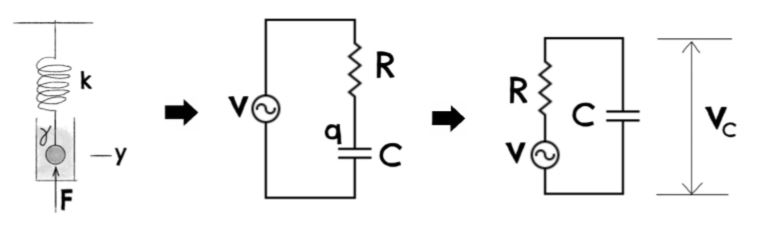
\includegraphics[width=\linewidth]{TSPEx4Q9.JPG}
\end{figure}
Use the classical fluctuation-dissipation theorem to show that $\langle|q(\omega)|^2\rangle=2k_BT\frac{\tau C}{1+\omega^2\tau^2}$ , where $\tau=RC$. Hence, obtain an expression for the spectrum of voltage noise $\langle|v(\omega)|^2\rangle$ across the series $R$-$C$ circuit. Compare your result to the expected Johnson noise $4Rk_BT$, noting that positive and negative frequencies contribute equally to Johnson noise in a frequency interval $[f,f + \Delta f]$.\\[5pt]
Calculate the voltage noise across the capacitor, $\langle|v_C(\omega)|^2\rangle$, and by integrating this check that the variance $\langle v_C^2\rangle$ is consistent with the equipartition theorem.\\[5pt]
Show that the power dissipated in the resistor equals the power supplied by the noise source.\\[5pt]
In a parallel $R$−$C$ circuit, the voltage noise spectrum across the known capacitor $C$ is measured at an unknown temperature $T$ for an unknown, temperature-dependent resistor $R(T)$. Outline how the measured voltage noise spectrum can be used to extract both temperature and resistance.
\end{qns}
\begin{ans}

\end{ans}
\newpage
\begin{qns}[Ratchet and pawl]
The famous ratchet and pawl machine, originally suggested by Smoluchowski in 1912 to be able to extract useful work from a thermal reservoir (against the Laws of Thermodynamics) is shown below. The pawl preventing the backward rotation of the wheel allows the energy transferred to the flaps from the thermal motion of surrounding gas to be rectified, i.e. only channelled in one direction.
\begin{figure}[H]
    \centering
    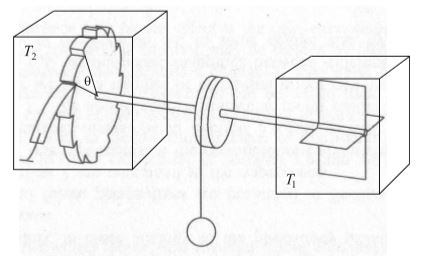
\includegraphics{TSPEx4Q10.JPG}
\end{figure}
If the energy required to lift the pawl and make one step of forward motion is $\varepsilon$ and the work against the external torque $L$ (e.g. from the lifted mass in the sketch) is $L\theta$, with $\theta$ the angle of single-step turn, show that the system is reversible if
$$\frac{\varepsilon+L\theta}{T_1}=\frac{\varepsilon}{T_2}$$
where $T_1$ and $T_2$ are the temperatures of the gas and the vanes, and of the ratchet wheel, respectively. As a result, prove that the Carnot condition for a reversible cycle holds, $Q_1/Q_2=T_1/T_2$, where $Q_1$ is the energy taken from the vanes and $Q_2$ the energy delivered to the wheel. 
\end{qns}
\begin{ans}

\end{ans}
\newpage
\begin{qns}[Diffusion]
Consider free Brownian particles diffusing along the axis $x\geq0$, so that there is a reflecting wall at $x = 0$. Also there is a `sink' at $x = L$ where the particles can escape from the system, so that the probability at that point is $P(L,t) = 0$ at any time.\\[5pt]
If the diffusion constant is $D$, estimate how long on average it would take for all the particles to escape from the system.
\end{qns}
\begin{ans}

\end{ans}
\end{document}